% !TeX spellcheck = en_US
\documentclass[12pt]{article}
\usepackage[unicode=true]{hyperref}
\usepackage[utf8x]{inputenc}
\usepackage{amsmath,amsthm,amsfonts,eucal}
\usepackage{graphicx}
\usepackage{placeins}


\title{Applications of the Fresnel Integrals}
\author{Jack Jones}
\date{March 17\th, 2019}


\newcommand\defbb[2]{\def#1{{\mathbb{#2}}}}
\newcommand\defbf[2]{\def#1{{\mathbf{#2}}}}
\newcommand\defcal[2]{\def#1{{\mathcal{#2}}}} % capital letters only
\newcommand\defrm[2]{\def#1{{\mathrm{#2}}}}
\newcommand\defsf[2]{\def#1{{\mathsf{#2}}}}
\newcommand\defvec[2]{\def#1{{\vec{#2}}}}
\def\vec{\mathbf}
\renewcommand\th[1][th]{$^{\text{#1}}$}
\newtheorem*{thm}{Theorem}

\let\C=\relax
\DeclareMathOperator\C{C} % \C(x) := \int_0^x cos(\pi/2*t^2) \d{t}
\defbb\CC{C} % complex numbers
\defrm\ud{d}
\def\d#1{{\,\ud#1\,}}
\newcommand\udfrac[2]{\ensuremath{\frac{\ud#1}{\ud #2}}}
\defrm\e{e}  % Euler's number
\DeclareMathOperator\erf{erf} % error function
\defsf\si{i} % \sqrt{-1}
\defbb\R{R}
\let\para=\S
\let\S=\relax
\DeclareMathOperator\S{S} % \S(x) := \int_0^x sin(\pi/2*t^2) \d{t}


\begin{document}\def§{{\ensuremath{\para}}}
\maketitle
\begin{abstract}

The Euler spiral is a well known mathematical curve which can be constructed, e.g.~by peeling an orange along a spiral with a kitchen knife.  Euler described it geometrically by a differential equation that sets the curvature linear to the arc length.  On the other hand Fresnel integrals arise naturally in the mathematical description of Fresnel diffraction.  We will study this in detail as a first application.

We further reproduce the theorem that Fresnel integrals are the mathematical solutions of the Euler spiral. We also study another major application: railway transition curve construction where one tries to find a railway track than can be traveled smoothly even at higher velocities.  We show that the transition curve construction has a simple solution in the Euler spiral.  For practical purposes, we need to draw the Euler spiral or segments of it explicitly which can be done using the Fresnel integrals.

In this sense we argue that the Euler spiral and the Fresnel integrals are two views of the same concept and are most fruitfully applied together.
\end{abstract}
\clearpage


\section{Introduction}
An Euler spiral is a famous curve whose curvature changes proportional to  its arc length. Taking the example of peeling an orange with a kitchen knife, one can either cut the skin vertically, or cut it along a spiral as the left-hand image in Figure~\ref{f:orangePeel} shows. The red lines marked on the orange refer to the route one can follow to peel the orange. Later, if we unfold the spiral strip and flatten it on a table, we will see a long curve which is curved differently at different positions. Imagine that we will now cut the peel with progressively thinner width of the strip, what we will obtain in the end is a long beautiful curve known as Euler spiral, as the right-hand image in Figure~\ref{f:orangePeel} shows. According to Alfred Gray, Euler spiral is ``one of the most elegant of all plane curves.'' \cite{ASG17}


\begin{figure}[h!]
	\centering
	\includegraphics[height=5cm]{orange.jpg} \hfill
	\includegraphics[height=5cm]{orangePeel.jpg}
	\label{f:orangePeel}
	\caption{Left: Peeling an orange in a spiral of height $1/N$.
		Right: The flattened orange peel that resembles an Euler spiral.  Photos taken from \cite{BH12}.
	}
\end{figure}

For a mathematician, an interesting question is whether there are any equations that can describe the corresponding shape of an Euler spiral. For this we consider the Fresnel integrals.  These are defined as integrals over some elementary functions which can however not be integrated in elementary functions.  These integrals occur naturally in the description of the optics of an illuminated straight edge (see Subsection~\ref{s:app1}).


\subsection{Definition of Euler Spiral}
The Euler Spiral, defined by the  linear relationship between curvature and arc length, was
first proposed as a problem of elasticity by James Bernoulli, then solved accurately by Leonhard Euler \cite{Lev08}.
The Euler spiral is a curve in the complex plane that has curvature proportional to the arc length.  Here the arc length $s(t)$ of a differentiable curve $(x(t),y(t))$ in the plane is defined by
\[  \left(\udfrac{s}{t}\right)^2 := \left(\udfrac{x}{t}\right)^2 +\left(\udfrac{y}{t}\right)^2.
\]  Note that the arc length is monotone increasing with the parameter $t$ of the curve.  For a nice curve, it is possible to rewrite the curve in the arc length, i.e.~$(x(s),y(s))$.

The curvature $\kappa$ of a smooth curve can be defined as 
\[  \kappa=\frac1R = x'y'' -x''y'
\] if we assume that the curve is parameterized in the arc length $s$ \cite{BH12}.  The meaning is that at a point $(x(s),y(s))$ we approximate the curve by a circle segment that touches in this point of at least second order.  Then $R$ is the radius of this touching circle and $\kappa$ its inverse.

According to \cite{BH12} the peel of the orange can be approximated as
\begin{equation}
  \kappa \sim s  \label{e:eulerSpiral}.
\end{equation}  This is the differential equation of the Euler curve.  The goal is to find all smooth curves $(x(s),y(s))$ whose curvature is in every point as described.

The question we want to answer is how to describe the solution of this differential equation explicitly.  Therefore we introduce the Fresnel integrals.


\subsection{Definition of the Fresnel Integrals}
The Fresnel sine and cosine integrals are represented as $\S(x)$ and $\C(x)$.  They are two integral functions that originate by applying the analysis of Fresnel diffraction phenomena. The mathematical equations are as follows:

\begin{align}
  \S(x) &:= \int_0^x  \sin\left(\frac\pi2 t^2\right) \d{t}, \label{e:FresnelS}\\
  \C(x) &:= \int_0^x \cos\left(\frac\pi2 t^2\right) \d{t}, \label{e:FresnelC}
\end{align}
where $x$ is a real number and $t$ is a real variable.   The coefficient $\pi/2$ is just for normalization.  In particular, when $x$ tends to infinity, $\S=\C=1/2$.  The important property is that the integrand is a trigonometric function in the square of the integration variable.  The result is that these integrals cannot be computed with analytic means, i.e.~the functions are transcendental \cite[p.195ff]{AS}.  This is in contrast to, e.g.
$$ \int_0^x (\sin t)^2 \d{t} = \frac12\int_0^x \left(1-\cos(2t)\right)\d{t} = \frac12x -\frac14\sin(2x).
$$  The first step comes from the double angle formula $\cos(2t)=1-2(\sin t)^2$ \cite{AS}.  There is however no square angle formula, i.e.~anything related to $\cos(t^2)$.


\subsection{Mathematical history}
If we trace the history of the Euler spiral and Fresnel integrals, we will find it under different authors, e.g.~Fresnel, Euler, Cornu and others.  This is because of the long history that Fresnel integral and the related Euler spiral have already left behind. They were discovered multiple times and under varying names during history.  One of the first occurrences is according to \cite{Lev08} by the French physicist J. Bernoulli in 1694.  Bernoulli approached many problems in elasticity theory at that time. One of them is a curve such that an ideal metal rod of this shape unwinds to a straight line when placed under load at the ends. He tried to find an explicit mathematical description of that curve, but it turned out that it is not that easy to do so at that time. In 1744, Swiss physicist and mathematician L. Euler is able to describe the same curve by a differential equation. This allows him to formulate a solution with integrals, namely what will later be called the Fresnel integrals.  37 years later, he computes the limiting points ($t\to\pm\infty$) of the curve and integrals which are $(\pm1/2,\pm1/2)$. In 1818, the French A.J. Fresnel who deals with many problems in wave optics and is unaware of the earlier results by Bernoulli and Euler discovers the Euler spiral independently and successfully applies it to the diffraction on a slit \cite{Lev08}.  He is also able to compute a couple of values numerically. With this finding he is able to establish the success of wave optics over particle optics which describes light as a transversal wave as opposed to the older idea by Newton who described light as consisting of particles.  In 1874 the French physicist M.A. Cornu followed similar ideas as Fresnel and is able to plot the curve accurately and proposes it as a graphical means for computing diffraction problems.  For that reason the Euler spiral is often also called Cornu spiral.


\section{Properties of the Fresnel Integrals}
The Fresnel integrals have many interesting mathematical properties. In this section, we will present some of them. 
\subsection{Basic properties}
\begin{enumerate}
\item The Fresnel integrals are odd, i.e.
\begin{align*}
	\S(-x) &= \S(x), & \C(-x) &= \C(x).
\end{align*}
\begin{proof}[Idea of proof]  The integrands $\sin(t^2)$ and $\cos(t^2)$ are even in $t$ and an anti-derivative $F(x)$ of an even function is odd if in addition $F(0)=0$.  The latter follows, because both integrals start at $t=0$.
\end{proof}
This means that the full graphs of $\S$ and $\C$ are point symmetric at the origin.  It is therefore enough to plot them for positive arguments.  In particular this implies $\C(0)=0=\S(0)$.

\item Their limits are according to \cite{AS}
\[  \lim_{x\to\pm\infty} \S(x) = \pm0.5,\qquad  \lim_{x\to\pm\infty} \C(x) = \pm0.5.
\]  Euler was first able to compute these limits from an analysis of the Fresnel integrals.  From the formulation as integral it is not obvious that the improper integrals (with unbounded domain) converge to a finite value of $1/2$.  However if we note that the integrand is oscillating with increasing amplitude ($\sin(t^2)=\sin(\omega t)$ for $\omega(t)=t$ increasing, and the analogue for $\cos(t^2)$), then it becomes plausible that the alternating positive and negative contributions from $t^2=k\pi$ to $t^2=(k+1)\pi$ (i.e.~lengths of the intervals $\sqrt{(k+1)\pi}-\sqrt{k\pi}$ for $k=0,1,2,\dots$) become smaller and smaller, asymptotically approaching 0.  By Leibniz criterion the whole integral should thus converge.

\item Since the integrals cannot be computed by elementary analytic means, an alternative is to compute them via power series.  Therefore we present the Taylor expansion as
\begin{align*}
  \S(x) &= \sqrt{\frac\pi2}\sum_{n\ge0} (-1)^nx^{4n+3}\frac{(\pi/2)^{2n+1}}{(2n+1)!(4n+3)}, \\
  \C(x) &= \sqrt{\frac\pi2}\sum_{n\ge0} (-1)^nx^{4n+1}\frac{(\pi/2)^{2n}}{(2n)!(4n+1)}.
\end{align*}
\begin{proof}[Idea of proof]  Start from the well known Taylor expansion of $\sin t = \sum_{n\ge0}$ $(-1)^n t^{2n+1}/(2n+1)!$ and $\cos t = \sum_{n\ge0} (-1)^nt^{2n}/(2n)!$, substitute $t\mapsto \tfrac\pi2 t^2$ and take the antiderivative for each summand.  The resulting series are $\S(t)$ and $\C(t)$, because the integral of an absolutely converging power series equals the absolutely converging power series of the integrals of the summands.
\end{proof}
In order to compute approximate numerical values for particular finite arguments, we would now sum up the Taylor series up to a certain degree $n$ such that the following term (for $n+1$ which is of the order of the error) is small compared to the required precision.  Unfortunately this means that we need to add more terms for larger arguments $x$.  The formulas are therefore not very helpful to compute the limit $x\to\pm\infty$.

\item From the power series it follows that the Fresnel integrals are analytic on the whole complex plane.  In particular they are entire complex functions.  This allows us to use the full machinery of complex analysis to discuss further properties of the integrals.

\item With these power series it is possible to draw the Fresnel integrals for real arguments Figure~\ref{f:graphFresnelIntegrals}.  Similar to the sine and cosine functions, the Fresnel integrals are oscillating.  However the distance between consecutive local maxima (or also consecutive local minima) are constantly decreasing.  This is as we already argued under the limit $x\to\infty$, because the integrands are alternatingly positive and negative for intervals of decreasing length.
\end{enumerate}
\begin{figure}[h!]
	\centering
	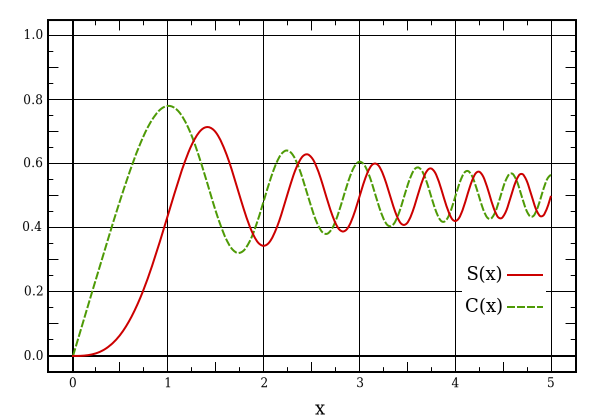
\includegraphics[width=0.4\textwidth]{Fresnel-Integrals-(Normalised).png}
	\label{f:graphFresnelIntegrals}
	\caption{Fresnel integrals \cite{wiki}.}
\end{figure}


\FloatBarrier
\subsection{Relation to the Euler spiral}\label{s:relation}
We will now formulate a major relation between the Fresnel integrals and the Euler spiral.  This was first observed by Euler in 1744.  Euler derived this property by constructing the solution of the differential equation \eqref{e:eulerSpiral} where he obtained what was later called Fresnel integrals \eqref{e:FresnelS} and \eqref{e:FresnelC}.
\begin{thm}  The curve $(x,y)=(\C(t),\S(t))$ is an Euler spiral.
\end{thm}
\begin{proof}  Let us start by showing that $t$ is the parameter of the arc length.  Consider therefore the derivatives
\begin{align*}
  \C'(t) &= \cos\left(\frac\pi2 t^2\right), &  
  \S'(t) &= \sin\left(\frac\pi2 t^2\right), \\
  \C''(t) &= -\frac\pi2\sin\left(\frac\pi2 t^2\right)\cdot 2t, &
  \S''(t) &= \frac\pi2\cos\left(\frac\pi2 t^2\right)\cdot 2t.
\intertext{Then}
  \left(\udfrac{s}{t}\right)^2 &= (C'(t))^2+(S'(t))^2 = 1
\end{align*}
i.e.~$t$ is the arc length $s$ of the curve.

Let us now consider the curvature
\begin{align*}
  \kappa &= x'y''-x''y' = C'(t)S''(t)-C''(t)S'(t) = \frac{\pi}{2}2t \sim t
\end{align*}  This completes the proof of the theorem.
\end{proof}

This theorem establishes two things.  First, the Fresnel integrals are particular solutions of the Euler spiral \eqref{e:eulerSpiral}.  This is particularly helpful for engineers, because in practical applications it is necessary to draw and compute the shape of the Euler spiral.

Secondly, the Euler spiral \eqref{e:eulerSpiral} has a solution for the whole parameter range $t\in\R$.  This property is not obvious, because usual existence and uniqueness theorems for ordinary differential equations \cite[Picard--Lindeloff theorem]{sim} either only work for linear differential equations or only state local existence and uniqueness.

\begin{figure}[h!]
	\centering
	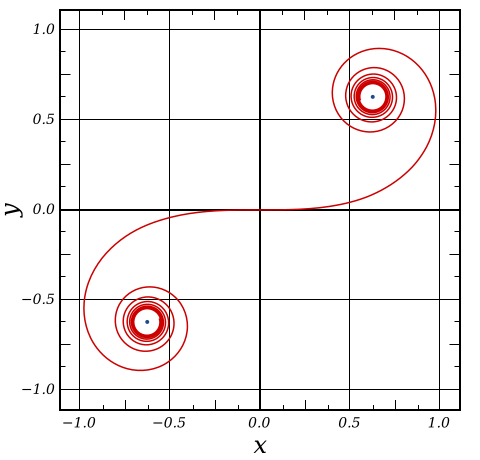
\includegraphics[width=0.5\textwidth]{eulerSpiral.png}
	\label{f:eulerSpiral}
	\caption{Euler spiral $(x,y)=(\C(t),\S(t))$ \cite{wiki}.}
\end{figure}


\subsection{Other expressions}
The Fresnel integrals are closely related to the error function which is defined as follows
$$  \erf(x) := \int_{-x}^x \exp(-t^2) \d{t}.
$$
Also this function is analytic and can therefore be expanded to the whole complex plane.  Here the integral for fixed endpoints is independent of the path by Cauchy's theorem \cite[p.~205]{Rudin}.

Now for the complex definition of exponential function
\begin{align}  \exp(x+\si y) &:= (\cos y +\si\sin y)\e^x \label{e:CFresnel}
\intertext{we obtain}
  \C(z)+\si\S(z) &= \int_0^z \exp\left(\si\frac\pi2 t^2\right)\d{t} 
\intertext{Here we do a substitution in the complex plane as $t'=\sqrt{\si\frac\pi2}t$, i.e.~$\d{t'}=\frac{1+\si}{\sqrt{2}}\sqrt{\frac\pi2}\d{t}$ and obtain}
  &= \frac{1-\si}{\sqrt{2}}\sqrt{\frac2\pi}\int_0^{\frac{1+\si}{\sqrt{2}}\sqrt{\frac\pi2}z} \exp(t^{\prime2}) \d{t'} = \frac12\sqrt{\frac2\pi}\,\frac{1-\si}{\sqrt2} \erf\left(\frac{1+\si}{\sqrt2}\,\sqrt{\frac\pi2} z\right).  \nonumber
\end{align}
Therefore we can say that the Fresnel integrals are the real and imaginary part of the complex error function.


\section{Applications of the Fresnel Integrals}
Fresnel Integrals and Euler spiral have applications in many fields of science. They occurred originally in the analysis of the diffraction of light. More recently, Euler spiral appears in the design of highways and railroad tracks, robot trajectory planning, and computer-aided design. In this section, we will describe two main applications of the Fresnel integrals in detail, namely the original Fresnel Diffraction and the railway construction. 


\subsection{Fresnel Diffraction}\label{s:app1}
\defbf\E{E}
\defbf\B{B}
\begin{figure}[h!]
	\centering
	\includegraphics[width=0.5\textwidth]{opticalSetting.png} \\
	% (2) \includegraphics[width=0.5\textwidth]{opticalParameters.png}
	\label{f:FresnelDiffraction}
	\caption{Fresnel diffraction after \cite[ch.~8.1]{Zim08}. Incoming parallel light waves from the left.  An aperture S' and an observation screen on the right in distance $D$.}
\end{figure}
Consider an optical construction as in Figure~\ref{f:FresnelDiffraction}: A monochromatic plane light wave of amplitude $\B$ and frequency $\omega>0$ enters from the left through a plane aperture $S'$.  The light that emerges from the aperture travels a horizontal distance $D$ until it hits an observation screen.  Mathematically this is described as follows \cite[ch.~7]{Zim08}.  The electric field strength $\E$ at a point $P$ with coordinates $(x,y,D)$ on the observation screen computes as
\[  \E(P) = \B\iint  \frac1\rho \exp\left(\si(k\rho-\omega t)\right) \d{S'}
\] where $\rho=\sqrt{(x-x')^2+(y-y')^2+D^2}$ is the distance of the aperture point $S'$ with coordinates $(x',y',0)$ from the observation point $P$.  $k=\omega/c$ is the wave number and $c>0$ the speed of light.  In the Fresnel approximation we assume that $|x-x'|/D\ll 1$ and $|y-y'|/D\ll 1$, but will not assume that the aperture itself is small compared to the wave length.  Therefore we expand in the lowest orders of $(x-x')/D$ and $(y-y')/D$ and obtain
\[  \E(P) \approx \B\frac{\exp\left(\si(kD-\omega t)\right)}{D} \iint \exp\left(\si(x'-x)^2k/2D +\si(y'-y)^2k/2D\right) \d{(x',y')}.
\]  If we combine the constant coefficient as $\E_0$ and assume a rectangular aperture of size $[x_0,x_1]\times[y_0,y_1]$, we obtain
\begin{align*}  \E(x,y) &\approx \E_0 \int_{u_0}^{u_1} \exp\left(\si\frac\pi2 u^2\right)\d{u} \int_{v_0}^{v_1} \exp\left(\si\frac\pi2 v^2\right) \d{v} 
\intertext{Here we see that integrals of the complex error function arise.  According to \eqref{e:CFresnel} we can compute that with the Fresnel integrals as}
  &= \E_0 \left[\C(u_1)+\si\S(u_1)-\C(u_0)-\si\S(u_0)\right] \left[\C(v_1)+\si\S(v_1)-\C(v_0)-\si\S(v_0)\right]
\end{align*} where $u_k:=\sqrt{\frac2{D\lambda}}(x_k-x)$, $v_k:= \sqrt{\frac2{D\lambda}}(y_k-y)$ for $k=0,1$ \cite[Eqns.~(8.34a\&b)]{Zim08} and $\lambda=2\pi/k$ is the wave length.  The intensity near a vertical edge ($y_0=-\infty$, $y_1=\infty$) results as
\[  I(x):= |\E|^2 = \frac{I_0}{2} \left[\left(\frac12-\C(u_0)\right)^2+\left(\frac12-\S(u_0)\right)^2\right].
\] See also \cite[Eqn.~(8.38)]{Zim08}.  This formula is the distance along the Euler spiral between the right point at $t=\infty$ and the left point at $t=u_0$.

Therefore Cornu proposed to use the Euler spiral as a nomogram to do intensity computations in wave optics.

\FloatBarrier 
\subsection{Railway  Construction}
When a train travels at speed $v$ on a circular path of radius $R$ the passengers experience a centripetal acceleration $a$ as
$$  a = v^2/R.
$$ When the train travels on a straight (horizontal) line with constant speed there is no acceleration.  However, in order to change the direction, we need to accelerate.  The first solution that comes to mind is to connect the initial and final straight segments by a circle.  But when the train passes this track at constant speed, the acceleration jumps from 0 for the straight segment ($1/R=0$) to some positive value ($a>0$, because $1/R>0$).  This sudden change of acceleration can be much discomfort.  The effect is small when, e.g.~the first trains, traveled at quite low speeds, but becomes much stronger when the speed increases ($a\sim v^2$).  Therefore increased speeds of trains triggered the quest for better designed tracks.  The problem is to find a transition curve from a straight tangential line segment to a circular segment.

Different approaches were taken to this. According to \cite{Lev08}, Mr. Gravatt was the first one who choose a sine curve for this transition around the year of 1828. Unlike a circle, the sine curve $y=\sin x$ has the curvature $\kappa=1/R=-\sin x/\left(1+(\cos x)^2\right)^{3/2}$ that changes continuously from $\kappa=0$ at $x=0$ to $\kappa=1$ at $x=\pi/2$ and back to $\kappa=0$ at $x=\pi$.

In 1880, Charles Crandall asked for priority for the ``true transition curve'' in the Railroad Gazette.  The problem is officially on Ellis Holbrook to be solved, however, Arthur Talbot was among the first to approach the problem mathematically.  He describes the problem and his solution in the introduction to ``The Railway Transition Spiral'' \cite{Tal99}.

Given the centripetal acceleration $a=v^2/R$, an obvious solution is to construct a curve whose curvature, $\kappa=1/R$, increases linearly with the traveled distance. This is the geometry of an Euler spiral \eqref{e:eulerSpiral}.

Rankine did not know of the solution of the geometry problem by Leonhard Euler.  Instead he proposed a cubic curve (a polynomial degree 3, $z(x)=ax^3+bx^2+cx+d$ with some adaptable coefficients $a,b,c,d$), an approximation of the exact solution for small angular changes.   We can compare this to a parabola approximating a circle near a point.

Marie Alfred Cornu (and later other civil engineers) also solved the problem of Euler spirals independently. Euler spirals are now-a-days widely used in railroad and highway construction, because they provide a smooth transition, i.e.~an easement, between a straight horizontal and an inclined track connected by a circular curve.


\section{Conclusion}
The Euler spiral is a well known mathematical curve which can be constructed, e.g.~by peeling an orange along a spiral with a kitchen knife.  Euler described it geometrically by a differential equation that sets the curvature linear to the arc length.  We showed that Fresnel integrals are the mathematical solutions of the Euler spiral. 

In this paper, we also studied two of its major applications: Fresnel diffraction in optics and a railway transition curve construction.  While the former leads directly to the Fresnel integrals, it turns out that its practical evaluation relies fruitfully on the Euler spiral.

We showed that the transition curve construction has a simple solution in the Euler spiral, because here the curvature changes linearly with the traveled distance (arc length).  But for practical purposes, we need to draw the Euler spiral or segments of it explicitly which can be done using the Fresnel integrals.

In this sense the Euler spiral and the Fresnel integrals are two views of the same concept and are most fruitfully applied together.


\bibliographystyle{alphasorteprint}
\bibliography{bibliography.bib}
\end{document}
